%!TEX root = ../thesis.tex

% \pagebreak[4]
% \hspace*{1cm}
% \pagebreak[4]
% \hspace*{1cm}
% \pagebreak[4]

\chapter{Mélange d'outils}

\graphicspath{ {Chapter2/Chapter2Figs/PNG/}
  {Chapter2/Chapter2Figs/PDF/} {Chapter2/Chapter2Figs/} }

Comme vu dans le chapitre précédent, la déformation appliquée par un
outil spécifique est soit locale, soit globale. Pourtant, sur un même
ensemble de points, un utilisateur pourrait souhaiter réaliser des
déformations à la fois locales et globales. C'est sur cette
problématique que les idées de mélange d'outils ont été
introduites. Pour simplifier la compréhension des déformations
appliquées, nous ne nous concentrons ici que dans le cas d'outils
déformant l'espace $\mathbb{R}^2$.

\section{Etat de l'art}

On peut citer \cite{JBPS11} comme étant les premiers à proposer une
méthode permettant de mélanger des outils de déformation de
différentes dimensions. C'est sur celui-ci que nous avons commencé à
travailler car les résultats nous semblaient proches de ce que nous
souhaitons réaliser. Une lecture approfondie de l'article nous a fait
comprendre que la méthode n'était pas celle que nous souhaitions. En
effet, s'ils semblent s'appuyer sur des outils ayant des dimensions
différentes en fonction des zones à déformer, la gestion interne
repose uniquement sur des déformations d'outils de dimension
topologique 0 (points). L'aspect "multidimensionnel" est donc
uniquement présent pour imposer des contraintes supplémentaires sur
les calculs de coordonnées. Par exemple pour des sommets reliés par
une arête les auteurs définissent que les coordonnées évoluent de
façon linéaire le long de cette arête. De plus, pour évaluer
l'influence d'un point de contrôle sur l'espace, la technique proposée
se base sur une diffusion (nécessitant donc une discrétisation de
l'espace). Or c'est quelque chose que nous souhaitons éviter à cause
du temps de calcul requis pour ces calculs.
\\

\cite{GPCP13} quant à eux, proposent une méthode permettant le mélange
d'outil de même dimension, en s'intéressant particulièrement aux cas
des déformations à base de cage.  Nous nous sommes intéressés à cet
article de par sa récente publication (2013), sa proximité avec
\cite{Hur12}, un travail réalisé par un étudiant en Master ISI en
2012, et de l'utilisation de cages de déformation, le modèle semblant
le plus utilisé ces dernières années parmi les outils de dimension
topologique 2 (surfaces). L'idée est de réaliser un pavage de
différentes cages collées ensemble le long de leurs arêtes sur tout
l'espace à déformer et de considérer la position d'un point de
l'espace, et pas seulement par rapport à sa cage \textit{propre} (à
comprendre la cage englobant le point de l'espace) mais aussi par
rapport aux cages adjacentes à celle-ci.

Contrairement au déformations à base de cage en général, la position
d'un point de l'espace n'est plus simplement constituée d'une
combinaison linéaire des positions des sommets de sa cage propre, mais
résulte d'une interpolation linéaire entre la position calculée par
rapport à la cage propre et aux différentes cages
\textit{jointure}. Une cage jointure correspond à l'union des cages
incidentes à un sommet de la cage propre. L'avantage de cette méthode
est de localiser les déformations en les limitant au voisinage de la
cage incidente au sommet déplacé. Mais en contrepartie on peut avoir
jusqu'à $n+1$ coordonnées différentes pour un même point de l'espace, où
$n$ correspond au nombre de sommets de la cage propre. Car
possiblement il se peut que tous les sommets d'une cage soient
incidents à d'autres cages. Ce qui au final fait perdre un des
intérêts de la méthode, au moins en partie, à savoir la réduction de
la complexité en temps de calcul des coordonnées.

Par ailleurs cette formulation cache d'autres fonctions qui résultent
d'un procédé empirique, dont le cheminement n'est pas expliqué dans
l'article, ce qui rend la compréhension de l'utilité de ces fonctions
assez difficile.

\section{Cheminement de l'article}
Dans un premier temps, nous avons voulu reproduire le cheminement de
\cite{GPCP13}, pour comprendre quelles étaient les motivations
derrière la définition de chaque fonction. Pour visualiser les
différentes fonctions, nous considérons dans nos exemples un outil
composé d'une grille de 2*2 faces, où chaque face représente une
cage. L'unique cage jointure de chaque face est donc la cage composée
de l'union des 4 cages initiales.

Nous nous sommes basés sur la formulation globale décrite par
l'article, qui exprime la position finale d'un point de l'espace comme
étant une interpolation linéaire de la position d'un sommet $p$ par
rapport à sa cage propre et du mélange de la position de $p$ par
rapport à chacun de ses cages jointure:

\begin{equation}
  p = \beta T(p)  + (1 - \beta) J(p),
  \label{MELgen}
\end{equation}

où $T(p)$ et $J(p)$ représentent la position du point p par rapport à
sa cage propre et au mélange des positions par rapport à chaque cage
jointure respectivement, tandis que $\beta$ représente la distance au
bord de la cage propre.

Le calcul de $\beta$ est proposé par l'article. Il s'agit de mesurer
la distance d'un point de l'espace par rapport à chaque arête à la
fois incidente à sa cage propre et à une autre cage. Pour éviter de
devoir calculer des distances euclidiennes, l'article propose de se
baser sur les coordonnées calculées pour chaque point $p$ par rapport
aux sommets de sa cage propre. Comme nous l'avons expliqué au début,
la position d'un point $p$ par rapport à une cage est calculée comme
étant une combinaison linéaire pondérée des positions des sommets de
cette cage. De ce fait, on peut considérer la distance de $p$ à un
sommet de la cage comme étant liée à la coordonnée qui a été associée
à ce sommet. Et par extension, on peut considérer la distance de $p$ à
une arête comme étant liée à la somme des coordonnées associées aux
sommets incidents de cette arête. Plus précisément, plus on est proche
d'une arête, plus la somme des coordonnées associées aux sommets
incidents à cette arête va être proche de 1. A l'inverse, plus on est
loin d'une arête, plus la somme des coordonnées associées aux sommets
de cette arête va être proche de 0. La distance à une arête correspond
donc au complément à 1 de la somme des coordonnées associées à chaque
sommet des arêtes incidentes à plusieurs cages :

\begin{equation}
  d_e~ = (1 - \sum_{v \in e} \lambda_v)
\end{equation}

Où $e$ correspond à une arête, $v$ un sommet de $e$ et $\lambda_v$ la
coordonnée associée au sommet v. L'article calcule $\beta$ comme étant
le produit de la distance de $p$ à chaque arête de la cage propre qui
sont aussi incidentes à d'autres cages :

\begin{equation}
  \beta = f(\prod_{e \in C} d_e)
\end{equation}

Où $f(x)$ est une fonction de lissage (Equation \ref{MELlis}),
permettant de faire varier la taille de la zone d'infuence du mélange,
tout en conservant un estompement progressif :

\begin{equation}
  f(x) = \frac{1}{2} sin(\pi(\frac{x}{h}-\frac{1}{2})) + \frac{1}{2}
  \label{MELlis}
\end{equation}
Où $h \in~ ]0,1]$ représente la zone d'influence de l'arête, ce qui
permet de délimiter la zone où le mélange de coordonnées doit être
fait (figure \ref{MELpar}). Sur la fonction en elle-même, l'influence
de $h$ correspond à une contraction, en passant du domaine [0,1] au
domaine [0,h] (Figure \ref{MELfon}).

\begin{figure}[ht]
  \begin{center}
    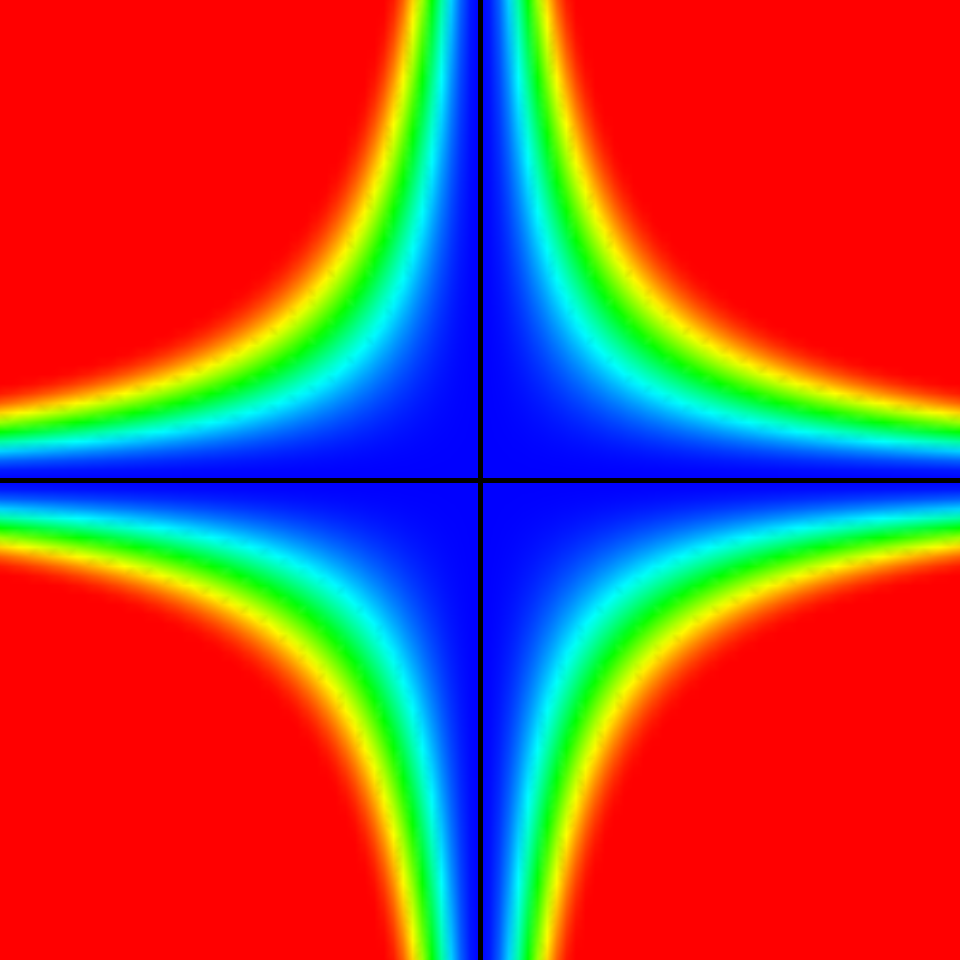
\includegraphics[scale=0.35]{starCage-0-2}
    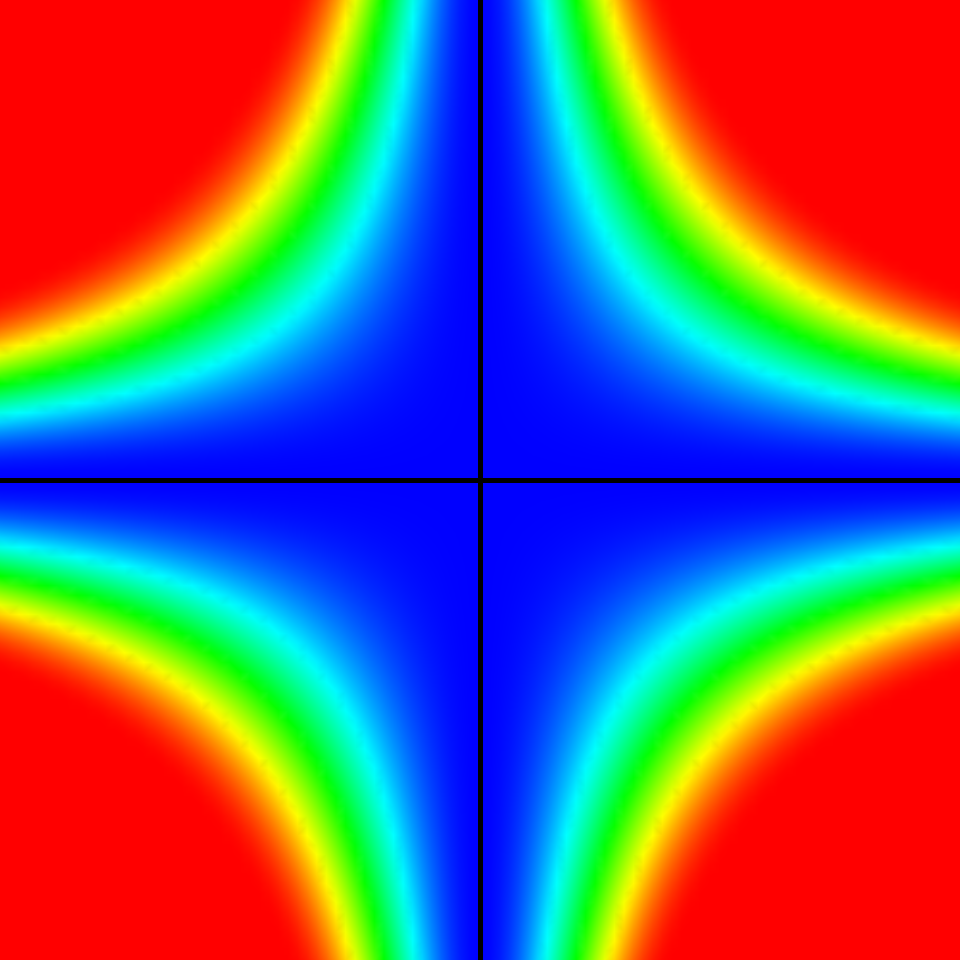
\includegraphics[scale=0.35]{starCage-0-4}
    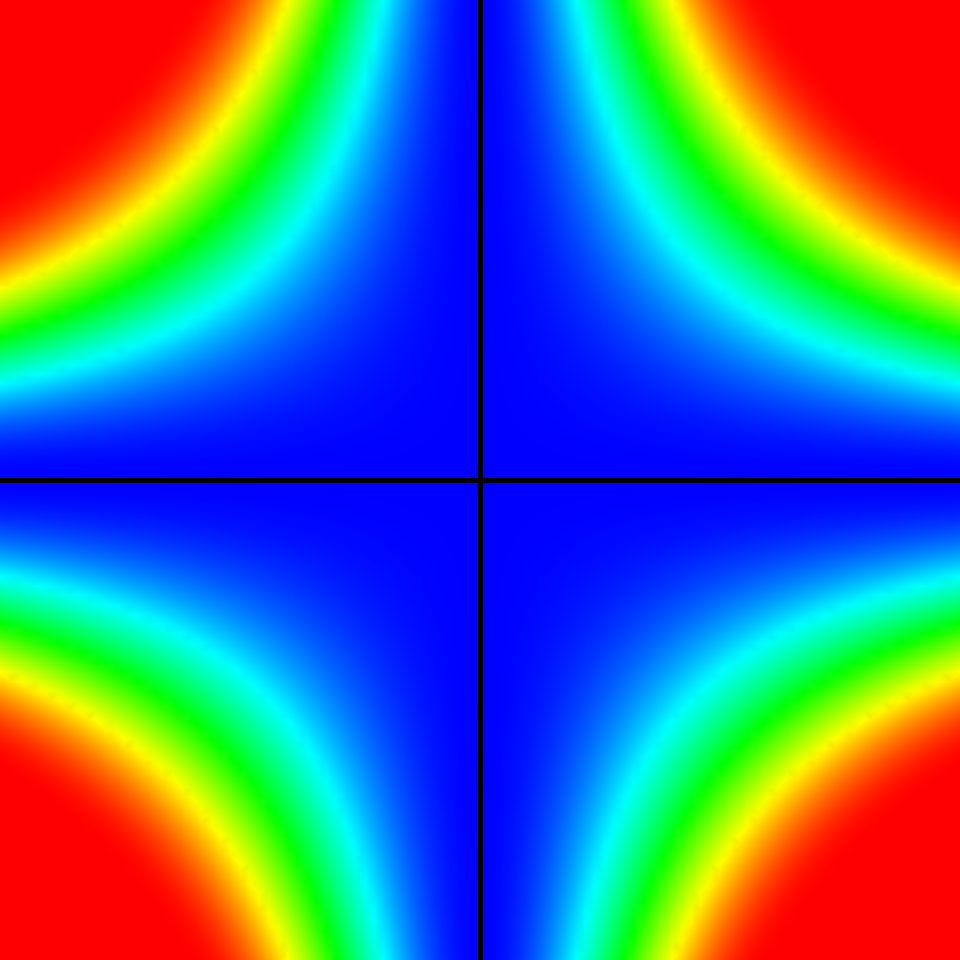
\includegraphics[scale=0.35]{starCage-0-6}
    \caption{Fonction de bordure calculée pour 4 cages (arêtes
      noires). Les variations de couleur représentent les variations
      de valeur de $\beta$ (la couleur bleu marine représentant une
      valeur de 0 et la couleur rouge une valeur de 1). En bleu les
      zones dites "de bordure" (i.e. points de l'espace proches d'une
      arête incidente à une autre cage). Valeurs de h : 0.2, 0.4 et
      0.6 pour les images à gauche, au centre et à droite
      respectivement.}
    \label{MELpar}
  \end{center}
\end{figure}

\begin{figure}[ht]
  \begin{center}
    \includegraphics{chapter2-attenuationfonction}
    \caption{Visualisation de la fonction f(x) pour différentes
      valeurs de h}
    \label{MELfon}
  \end{center}
\end{figure}

Comme $0 \leq \beta \leq 1$, on peut considérer $\beta$ comme le
pourcentage d'utilisation des coordonnées calculées par rapport à la
cage propre. D'après l'équation \ref{MELgen}, lorsque $\beta$ vaut 0
(i.e. $p$ se trouve sur une arête de la cage), la position de $p$
dépend uniquement de la coordonnée calculée par rapport à la cage
jointure.

C'est là qu'apparaît le premier problème : Dans la configuration
choisie (grille de 2*2 cages), toutes les cages sont incidentes à un
même sommet $s$. De ce fait, la zone autour des arêtes incidentes à ce
sommet est fortement influencée par l'unique cage jointure composée de
l'union des 4 cages. Afin que la cage jointure reste un polygone, $s$
ne doit pas être considéré comme un sommet de la cage jointure, car il
fait partie de l'intérieur de celle-ci. L'équation \ref{MELgen} nous
indique que les zones les plus proches des arêtes ne sont influencées
que par la cage jointure. Et que, par conséquent, $s$ n'a aucune
influence sur ces points. On peut voir sur la figure \ref{MELjoi} que
la déformation engendrée par le déplacement de $s$ n'est pas du tout
celle attendue.

\begin{figure}[ht]
  \begin{center}
    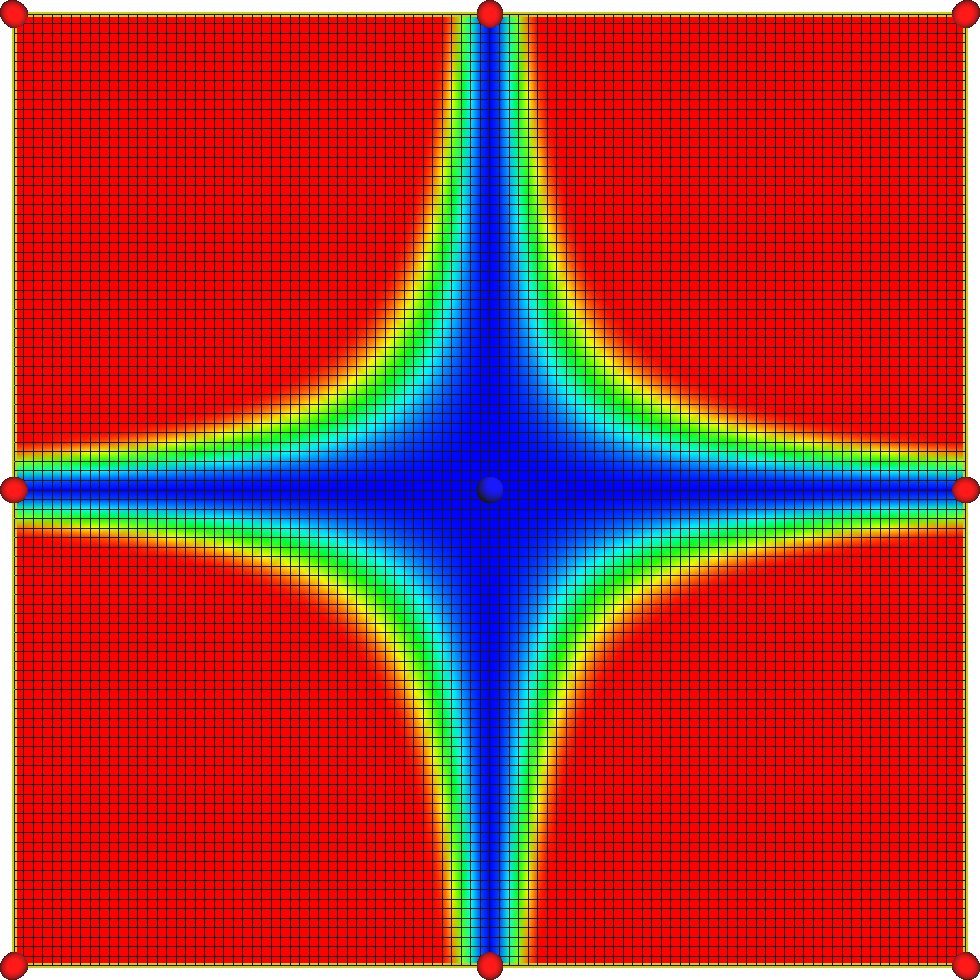
\includegraphics[scale=0.35]{starCage-jointure}
    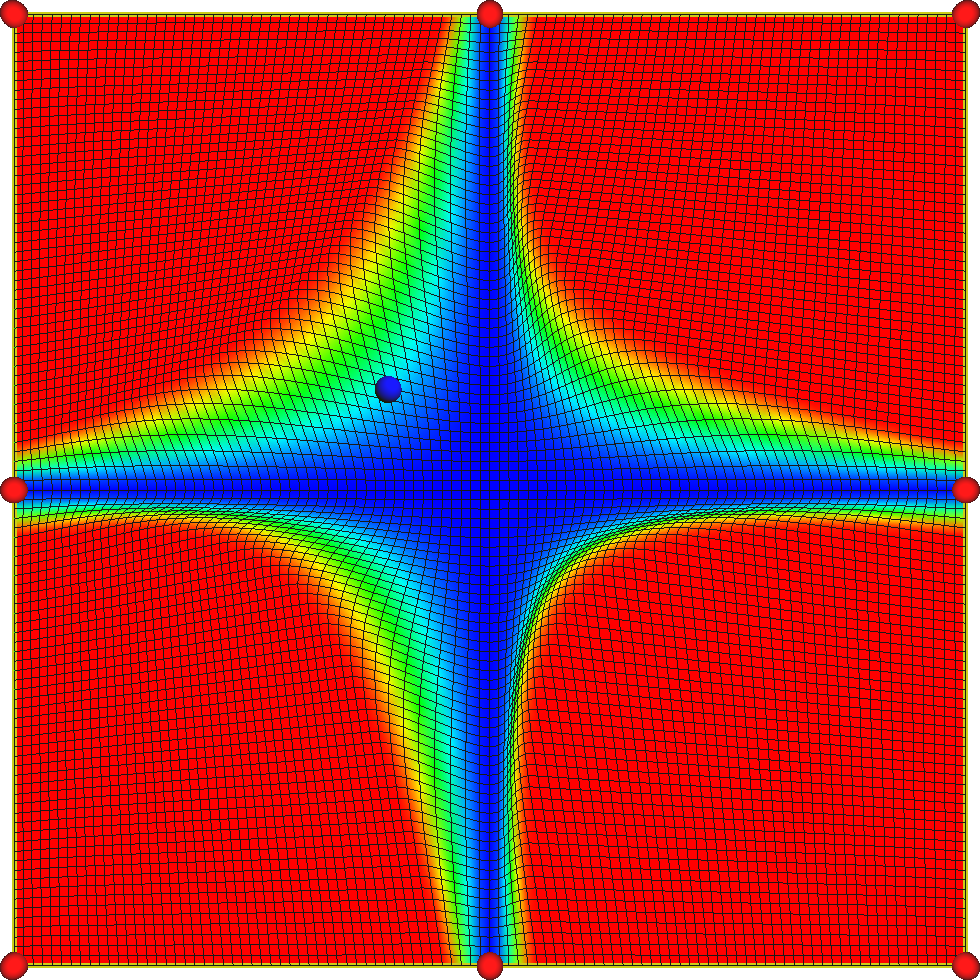
\includegraphics[scale=0.35]{starCage-jointure-deformation}
    \caption{A gauche la grille avant déformation et à droite la même
      grille après déplacement de $s$. Les boules rouges représentent
      les sommets de la cage jointure et la boule bleue représente le
      sommet $s$. Les zones en bleu ne sont pas modifiées par la
      translation de $s$.}
    \label{MELjoi}
  \end{center}
\end{figure}

De là, apparaît dans l'article la nécessité de rajouter un
comportement spécifique pour ces fameux sommets qui font partie de
l'intérieur de leur cage jointure. Ils résolvent ce problème au
travers de l'expression d'une déformation à base de points, associée
au sommet $s$. A partir de là, nous comprenons que la méthode proposée
\cite{GPCP13} n'est que le résultat d'une suite de résolutions de cas
spécifiques. Ce qui ne nous intéresse pas, car un de nos critères
principaux est l'utilisation d'une formulation simple permettant
d'exprimer les coordonnées de chaque point de façon claire. De plus,
cette méthode semble difficilement associable avec une méthode
multidimensionnelle, car elle se base sur une fusion d'outils (l'union
des cages de déformation), ce qui ne semble pas être directement
applicable pour des outils de différentes dimensions.

Nous pouvons néanmoins relever l'avancée qu'apporte cet article dans
le domaine des déformations à base de cages. En effet, grâce au
mélange de plusieurs cages, les déformations peuvent être locales,
tout en ayant un faible nombre de sommets composant les cages. De
plus, la possibilité d'utiliser conjointement plusieurs systèmes de
coordonnées différents permet de choisir le plus adapté aux
différentes déformations à effectuer.

C'est pour ça que la méthode qui suit s'inspire de cet article, en
gardant à l'esprit cette idée de localisation de la déformation et de
minimisation du temps de calcul des coordonnées.

\section{Méthode proposée}
Dans le cadre de ce stage, l'idée est de considérer des coordonnées
\textit{étendues} pour chaque cage, au lieu de considérer des unions
de cages, et de réaliser un mélange de coordonnées pour les points de
l'espace qui sont sous l'influence de plusieurs cages. On se base ici
sur le fait que les coordonnées MVC sont définies non seulement à
l'intérieur, mais aussi à l'extérieur du polygone de contrôle.

Pour vérifier la possibilité de réalisation d'une telle méthode, nous
avons commencé par travailler sur un exemple simple, une cage unique
déformant les points de l'espace à la fois à l'intérieur et à
l'extérieur grâce aux coordonnées MVC. Il s'agissait de voir le
comportement de la déformation, afin de savoir s'il était possible de
calculer des coordonnées à la fois à l'intérieur et à l'extérieur de
la cage, tout en permettant un passage lisse de l'un à l'autre. Car
dans la littérature, les coordonnées n'ont été utilisées que pour
déformer des points à l'intérieur du polygone et jusqu'à son bord.

Il se trouve que les coordonnées MVC sont $C^\infty$ partout, sauf au
niveau des sommets du polygone de contrôle, où elles ne sont que $C^0$
(Corrolaire 4.8 \cite{HF06}). De plus, à l'extérieur de la cage, on
peut constater que les coordonnées calculées ne diminuent pas quand la
distance d'un de point de l'espace augmente. Ceci est dû à la
partition de l'unité, qui est une propriété des coordonnées
barycentriques généralisées. Cette propriété est induite par la
normalisation des coordonnées associées à chaque sommet (Equation
\ref{MELnor}).

\begin{equation}
  \lambda_i(p) = \frac{w_i(p)}{\sum_{j=0}^n w_j(p)}
  \label{MELnor}
\end{equation}

Cette formule définit que la somme des coordonnées associées à chaque
sommet de la cage, pour un point $p$ donné, doit valoir 1 (Equation
\ref{MELsum}) :

\begin{equation}
  \sum_{i=0}^n \lambda_i(p) = 1
  \label{MELsum}
\end{equation}

Pour expliquer en quoi cela pose un problème, regardons la
construction des coordonnées MVC pour un point $p$ donné. Dans un
premier temps on évalue l'influence de chaque sommet $v_i$, dont le
calcul se fait par rapport au sommet voisins $v_{i-1}$ et $v_{i+1}$ :

\begin{equation}
  w_i(p) = \frac{tan(\alpha_{i-1}(p)/2) + tan(\alpha_{i}(p)/2)}{\|v_i - p\|}
\end{equation}

où $w_i(p)$ représente la coordonnée (avant normalisation) associée au
sommet $v_i$ pour le point $p$ et $\alpha_i(p)$ l'angle en $p$ du
triangle $[p,v_i,v_{i+1}]$ (Figure \ref{MELmvc}).

\begin{figure}[ht]
  \begin{center}
    \includegraphics{chapter2-pstricks}
    \caption{Visualisation du calcul de la coordonnée du point $p$ par
      rapport au sommet $v_i$}
    \label{MELmvc}
  \end{center}
\end{figure}

Les $w_i$ sont ensuite normalisés (Equation \ref{MELnor}), afin
d'obtenir des coordonnées contenus dans le domaine [0,1]. Le problème
est lié à cette normalisation, car quand on éloigne un point $p$ de la
cage, si les $w_i(p)$ tendent vers 0 quand la distance $\|v_i - p\|$
tend vers l'infini, leur somme aussi tend vers 0. De ce fait, les
points extrémement éloignés de la cage seront aussi fortement
influencés par les déformations appliquées sur la cage. On voit donc
la nécessité de définir des zones d'influence (avec un estompement
progressif de l'influence des coordonnées calculées) autour de chaque
cage, afin de limiter leur champ d'action.

Il existe aussi des problèmes avec les différentes méthodes de calcul
des coordonnées. Premièrement, contrairement à la technique proposée
par \cite{GPCP13}, notre méthode ne pourrait pas utiliser de
\textit{HC} (Coordonnées Harmoniques, définies par \cite{JMDGS07}),
car celles-ci ne sont pas définies à l'extérieur de la cage. Ce n'est
pas un problème en soit, car cette technique nécessite une
discrétisation de l'espace, or la minimisation du temps de calcul des coordonnées est
une de nos contraintes. Concernant les \textit{MVC} et les \textit{GC}
(Coordonnées de Green, définies par \cite{LLC08}), si elles sont bien
définies dans $\mathbb{R}^2$, la fonction résultant de la déformation
n'est pas dérivable sur tout le domaine (Figure \ref{SURcoo}). De ce
fait, des artefacts apparaissent au niveau des points de l'espace se
situant à proximité des sommets de la cage. Ce problème n'est pas
encore réglé au moment de l'écriture de ce rapport, mais c'est le
sujet des recherches et réflexions actuelles.

\begin{figure}[ht]
  \begin{center}
    \begin{tabular}{|l|c|c|c|}
      \hline
      \textbf{Domaine} & MVC & Harmoniques & Green\\
      \hline
      \textbf{Intérieur} & \textcolor{OliveGreen}{$C^\infty$} 
      & \textcolor{OliveGreen}{$C^\infty$} 
      & \textcolor{OliveGreen}{$C^\infty$} \\
      \hline
      \textbf{Bord} & \textcolor{Red}{$C^0$} 
      & \textcolor{Red}{$C^0$} 
      & \textcolor{Red}{$C^0$} \\
      \hline
      \textbf{Extérieur} & \textcolor{OliveGreen}{$C^\infty$} 
      & \textcolor{Red}{$C^0$}
      & \textcolor{OliveGreen}{$C^\infty$} \\
      \hline
    \end{tabular}
    \caption{Continuité de différentes méthodes de calcul des
      coordonnées (d'après \cite{GPCP13})}
    \label{SURcoo}
  \end{center}
\end{figure}